%\documentclass{acmsmall}
\documentclass[10pt, conference]{./IEEEtran}
\usepackage[pdftex]{graphicx}
\usepackage{url}
\usepackage{ifthen}
\usepackage{amsmath}
\usepackage[ruled]{algorithm2e}
\renewcommand{\algorithmcfname}{ALGORITHM}
\SetAlFnt{\small}
\SetAlCapFnt{\small}
\SetAlCapNameFnt{\small}
\SetAlCapHSkip{0pt}

\begin{document}

%\markboth{Scharfglass et al.}{Breaking weak 1024-bit RSA keys with CUDA}

\title{Breaking weak 1024-bit RSA keys with CUDA}

\author{\IEEEauthorblockN{Kerry Scharfglass, Darrin Weng,
Joseph White, Christopher Lupo}
\IEEEauthorblockA{Computer Science Department\\
  California Polytechnic State University\\
  San Luis Obispo, CA\\
  Email: \url{{kscharfg,dweng,jwhite09,clupo}@calpoly.edu}}
}

\maketitle

\begin{abstract}
   An exploit involving the \textit{greatest common divisor} (GCD) of RSA 
   moduli was recently discovered \cite{lenstra:ron}. This paper presents
   a tool that can efficiently and completely compare a large number of 
   1024-bit RSA public keys, and identify
   any keys that are susceptible to this weakness.
   NVIDIA's \textit{graphics processing units} (GPU) and the CUDA 
   massively-parallel programming model are powerful tools that can be used to 
   accelerate this tool. Our method using CUDA has a measured performance 
   speedup of 27.5 compared to a sequential CPU implementation, making it 
   a more practical method to compare large sets of keys.
   A computation for finding GCDs between 200,000 keys, i.e., 
   approximately 20 billion comparisons, was completed in 113 
   minutes, the equivalent of approximately 2.9 million 
   1024-bit GCD computations per second.
\end{abstract}

%\terms{Performance, Security}

\begin{IEEEkeywords}
CUDA, RSA, greatest common divisor, parallel computation
\end{IEEEkeywords}

\section{Introduction}
RSA is a public key encryption scheme which relies on the difficulty of 
factoring large numbers. The algorithm is prevalent throughout security, 
specifically it is used for many web-security applications. An RSA public key is 
comprised of a modulus $n$ of specified length (the product of primes $p$ and 
$q$), and an exponent $e$. The length of $n$ is given in terms of bits, thus 
the term ``1024-bit RSA key" refers to the number of bits which make up this 
value. The associated private key uses the same $n$, and another value $d$ such 
that $d \cdot e = 1 \:\text{mod} \;\phi(n)$ where $\phi(n) = (p - 1) \cdot (q - 1)$\cite{rsa}.
Ideally, given the number of possible primes that may be used to construct a 
1024-bit modulus, no random number generators should reuse either prime. Thus, 
the likelihood of either $p$ or $q$ being repeated in a set of keys should be 
approximately 0. An individual key may be considered secure by itself, but when 
compared to other keys, might exhibit a weakness which allows each key's 
$d$ to be calculated entirely from public information.

When considering two keys, a weakness exists when the greatest common 
divisor of both moduli, $n_1$ and $n_2$, is greater than 1. If $GCD(n_1, 
n_2) = p$, then $p$ must be a shared prime factor of $n_1$ and $n_2$. Thus, 
$q_1 = \frac{n_1}{p}$ and $q_2 = \frac{n_2}{p}$. Once $p$ and $q$ are known, 
$d_1$ and $d_2$ can be directly calculated, yielding both private key pairs.

This weakness is discussed in \cite{lenstra:ron}, which showed a 
significant number of existing RSA keys were susceptible to this exploit. The 
primary goal of our work was to speedup the most computationally intensive 
part of their process by implementing the GCD comparisons of RSA 1024-bit keys 
using NVIDIA's CUDA platform.

To aid in accomplishing this goal, the work in \cite{fujimoto2009high} was 
expanded and adapted to compare all combinations of keys in a given set. In 
comparison to their work, larger sections of the overall program were able to 
be executed in parallel, resulting in further speedup.

\section{Related Work}
The work documented in \cite{lenstra:ron} served as inspiration for this work.
Here, Lenstra et al. performed a sanity check of a wide array of public RSA keys 
contained in SSL certificates and SSH host keys. Their discovery that a 
significant fraction of these keys (roughly 0.2\%) were weak led to our 
desire to parallelize their investigation, in order to make it as efficient as 
possible with commodity hardware. 

The CUDA implementation of the binary GCD algorithm that was built upon 
(cf. \cite{fujimoto2009high}) is an important example of similar work being 
done. On a fundamental level, our work mirrors theirs as we based the core of 
our algorithm on their work, specifically 1024-bit GCDs were calculated in 
parallel using CUDA. However, we expanded its relevance with modifications in 
order to automatically divide and parallelize lists of large values to compare. 

Another example of work that makes use of the GPU for security applications is 
solving discrete logarithms as presented in \cite{henrysolving}. 
A set of large-precision operations (768-bit) was necessary for this work, and 
was thus implemented in CUDA. This was similar to our own starting point due to 
the currently-limited CUDA support for large-precision numbers. Because these 
large values have numerous applications in computer security, the work shown 
here displays another component of computer security where parallelizing work 
with the large values can be highly advantageous. 

Our work is an example of an amalgamation of other related works. It functions 
as a supplement to the other materials mentioned here, and provides another 
example of a computer security application that significantly benefits from 
using parallelization with commodity Single Instruction, Multiple Data (SIMD) 
multiprocessors. What sets it apart is its use of 1024-bit RSA keys and the 
method of parallelization implemented. 

\section{Overview of CUDA}
CUDA is a platform that provides a set of tools along with the ability to 
write programs that make use of NVIDIA's GPUs (cf. 
\cite{nvidia2012programming}). These massively-parallel hardware devices are 
capable of processing large amounts of data simultaneously, allowing 
significant speedups in programs with sections of parallelizable code using 
the SIMD model. The platform allows for various arrangements of threads to 
perform work, based on the developer's decomposition of the problem. Our 
solution to the problem presented in this paper is discussed in 
$\S$\ref{sec:GridOrg}. In general, individual threads are grouped into up-to 
3-dimensional blocks to allow sharing of common memory between threads. These 
blocks can then be organized into a 2-dimensional grid. 

The GPU breaks the total number of threads into groups called warps, which 
consist of 32 threads that will be executed simultaneously on a single
\textit{streaming multiprocessor} (SM). The GPU consists of several SMs which 
are each capable of executing a warp. Blocks are scheduled to SMs until all 
allocated threads have been executed. 

There is also a memory hierarchy on the GPU. There are 3 types of memory 
that are relevant to this work: global memory is the slowest and 
largest; shared memory is much faster, but also significantly smaller; and 
a limited number of registers that each SM has access to. Each thread in a
block can access the same section of shared memory.

\section{Algorithm Description}
\subsection{Binary GCD}
Binary GCD is a well known algorithm for computing the greatest common divisor 
of two numbers. Instead of relying on costly division operations like Euclid's 
algorithm, bitwise shifts are employed. The implementation
presented in this paper follows the outline displayed in Algorithm~\ref{alg:binGCD}.

\begin{algorithm}
   \KwIn{$x$ and $y$: two integers.}
   \KwOut{The greatest common divisor of $x$ and $y$.}
   \nl\Repeat {$GCD(x, y) = GCD(0, y) = y$} {
      \nl\uIf {$x$ and $y$ are both even} {
         \nl$GCD(x, y) = 2 \cdot GCD(\frac{x}{2}, \frac{y}{2})$\;
      }\nl\uElseIf{$x$ is even and $y$ is odd} {
         \nl$GCD(x, y) = GCD(\frac{x}{2}, y)$\;
      }\nl\uElseIf {$x$ is odd and $y$ is even} {
         \nl$GCD(x, y) = GCD(\frac{y}{2}, x)$\;
      }\nl\ElseIf {$x$ and $y$ are both odd} {
         \nl\eIf {$x \geq y$} {
            \nl$GCD(x, y) = GCD(\frac{x - y}{2}, y)$\;
         }{
            \nl$GCD(x, y) = GCD(\frac{y - x}{2}, x)$\;
        }
      }
   }
   \caption{Binary GCD algorithm outline}
   \label{alg:binGCD}
\end{algorithm}

\subsection{Parallel Functions}
To accomplish Algorithm \ref{alg:binGCD} using CUDA, the following three 
functions had to parallelized: shift, subtract, and greater-than-or-equal. As 
outlined in \cite{fujimoto2009high}, each 1024-bit number is divided across one 
warp so that each thread has its own 32-bit integer. 

The parallel shift function is straightforward: each thread is given an 
equal-sized piece of the large-precision integer. Then each thread except for 
Thread 0 grabs a copy of the integer at \texttt{threadID  - 1}.
The variable \texttt{threadID} refers to a value between 0 and 31 and corresponds 
to a thread in a warp. Each thread shifts its value once and 
uses its copy of the adjacent integer to determine if a bit has shifted 
between threads. This procedure is outlined in Algorithm \ref{alg:parShift}.
\begin{algorithm}
   \KwIn{$x[32]$ is a 1024-bit integer represented as an array of 32 \texttt{int}s, $threadID$ is the 0-31 index of the thread in warp.}
   \nl\eIf {$threadID \neq 0$} {
      \nl$temp\gets x[threadID - 1]$\;
   }{
      \nl$temp\gets 0$\;
   }
   \nl$x\gets x>>1$\;
   \nl$x\gets x \:\text{OR}\: (temp << 31)$\;
   \caption{Parallel right shift}
   \label{alg:parShift}
\end{algorithm}

The parallel subtract uses a method called \emph{carry skip} from 
\cite{fujimoto2009high}. First, each thread subtracts its piece and sets the 
``borrow" flag of \texttt{threadID - 1} if an underflow occurred. Next, each 
thread checks if it was borrowed from and if so, decrements itself and clears the 
flag. Then, if another underflow occurs, the borrow flag at \texttt{threadID 
- 1} will be set. This continues until all the borrow flags are cleared. An 
outline can be found in Algorithm \ref{alg:parSub}.

\begin{algorithm}
   \KwIn{$x$ and $y$: two 1024-bit integers, $threadID$ is the 0-31 index of the thread in warp.}
   \nl$x[threadID]\gets x[threadID]-y[threadID]$\;
   \nl\If {underflow} {
      \nl set $borrow[threadID - 1]$\;
   }
   \nl\Repeat {all $borrow$ flags are cleared} {
   \nl\If {$borrow[threadID]$ is set} {
      \nl$x[threadID]\gets x[threadID] - 1$\;
         \nl\If {underflow} {
            \nl set $borrow[threadID - 1]$\;
         }
         \nl clear $borrow[threadID]$\;
      }
   }
   \caption{Parallel subtract using ``carry skip"}
   \label{alg:parSub}
\end{algorithm}

The parallel greater-than-or-equal has each thread check if its integers are 
equal. If this is the case, then it sets a position variable shared by the warp 
to the minimum of its \texttt{threadID} and the current value stored in the position variable.
This is done atomically to ensure the correct value is stored. Finally, all 
the threads do a greater-than-or-equal comparison with the integers specified
by the position variable. This function is outlined in Algorithm \ref{alg:parGEQ}.
\begin{algorithm}
   \KwIn{$x$ and $y$: two 1024-bit integers, $threadID$ is the 0-31 index of the thread in warp.}
   \KwOut{$True$ if $x \geq y$; else $False$.}
   \nl\If {$x[threadID] \neq y[threadID]$} {
      \nl$pos\gets \text{atomicMin}(threadID, pos)$\;
   }
   \nl\Return $x[pos] \geq y[pos]$
   \caption{Parallel greater-than-or-equal-to}
   \label{alg:parGEQ}
\end{algorithm}

\subsection{Computational Complexity}
The computational complexity of the binary GCD algorithm has been shown by 
Stein and Vall$\acute{\text{e}}$e (cf. \cite{stein1967computational}, 
\cite{vallee1998complete}) to have a worst case complexity of $\mathcal{O}(n^2)$ 
where $n$ is the number of bits in the integer. The worst case is produced 
when each iteration of the algorithm shifts one of its arguments only once. 
Since for this application $n$ is fixed at 1024 bits, the complexity of a 
single GCD calculation can be considered to be constant time for the worst case.

To compare all the keys together, the amount of GCDs that must be calculated 
grows at a rate of $k^2$, where $k$ is the number of keys.

\subsection{Theoretical Speedup}
Maximum speedup is defined as follows:
\begin{equation}
   \mbox{Max Speedup} = \frac{1}{1 - P}
   \label{eq:speed}
\end{equation}

where $P$ is the percentage of the program's execution that can be parallelized.
This percentage is a function of the number of keys the program needs to 
process, and is calculated in Equation \ref{eq:percent}.
\begin{equation}
P = \frac{t \cdot g}{t \cdot g + r \cdot k}
   \label{eq:percent}
\end{equation}
where
\begin{itemize}
   \item $t$ = time to process a single GCD
   \item $g$ = total number of GCD calculations
   \item $r$ = time to read a single key
   \item $k$ = total number of keys
\end{itemize}

Since $g$ will increase significantly more rapidly than $k$, $P$ (based on 
equation \ref{eq:percent}) will approach $1$ as $k$ approaches 
$\infty$. This relationship can be observed in Figure \ref{fig:parPercent}.

\begin{figure}
   \centering
   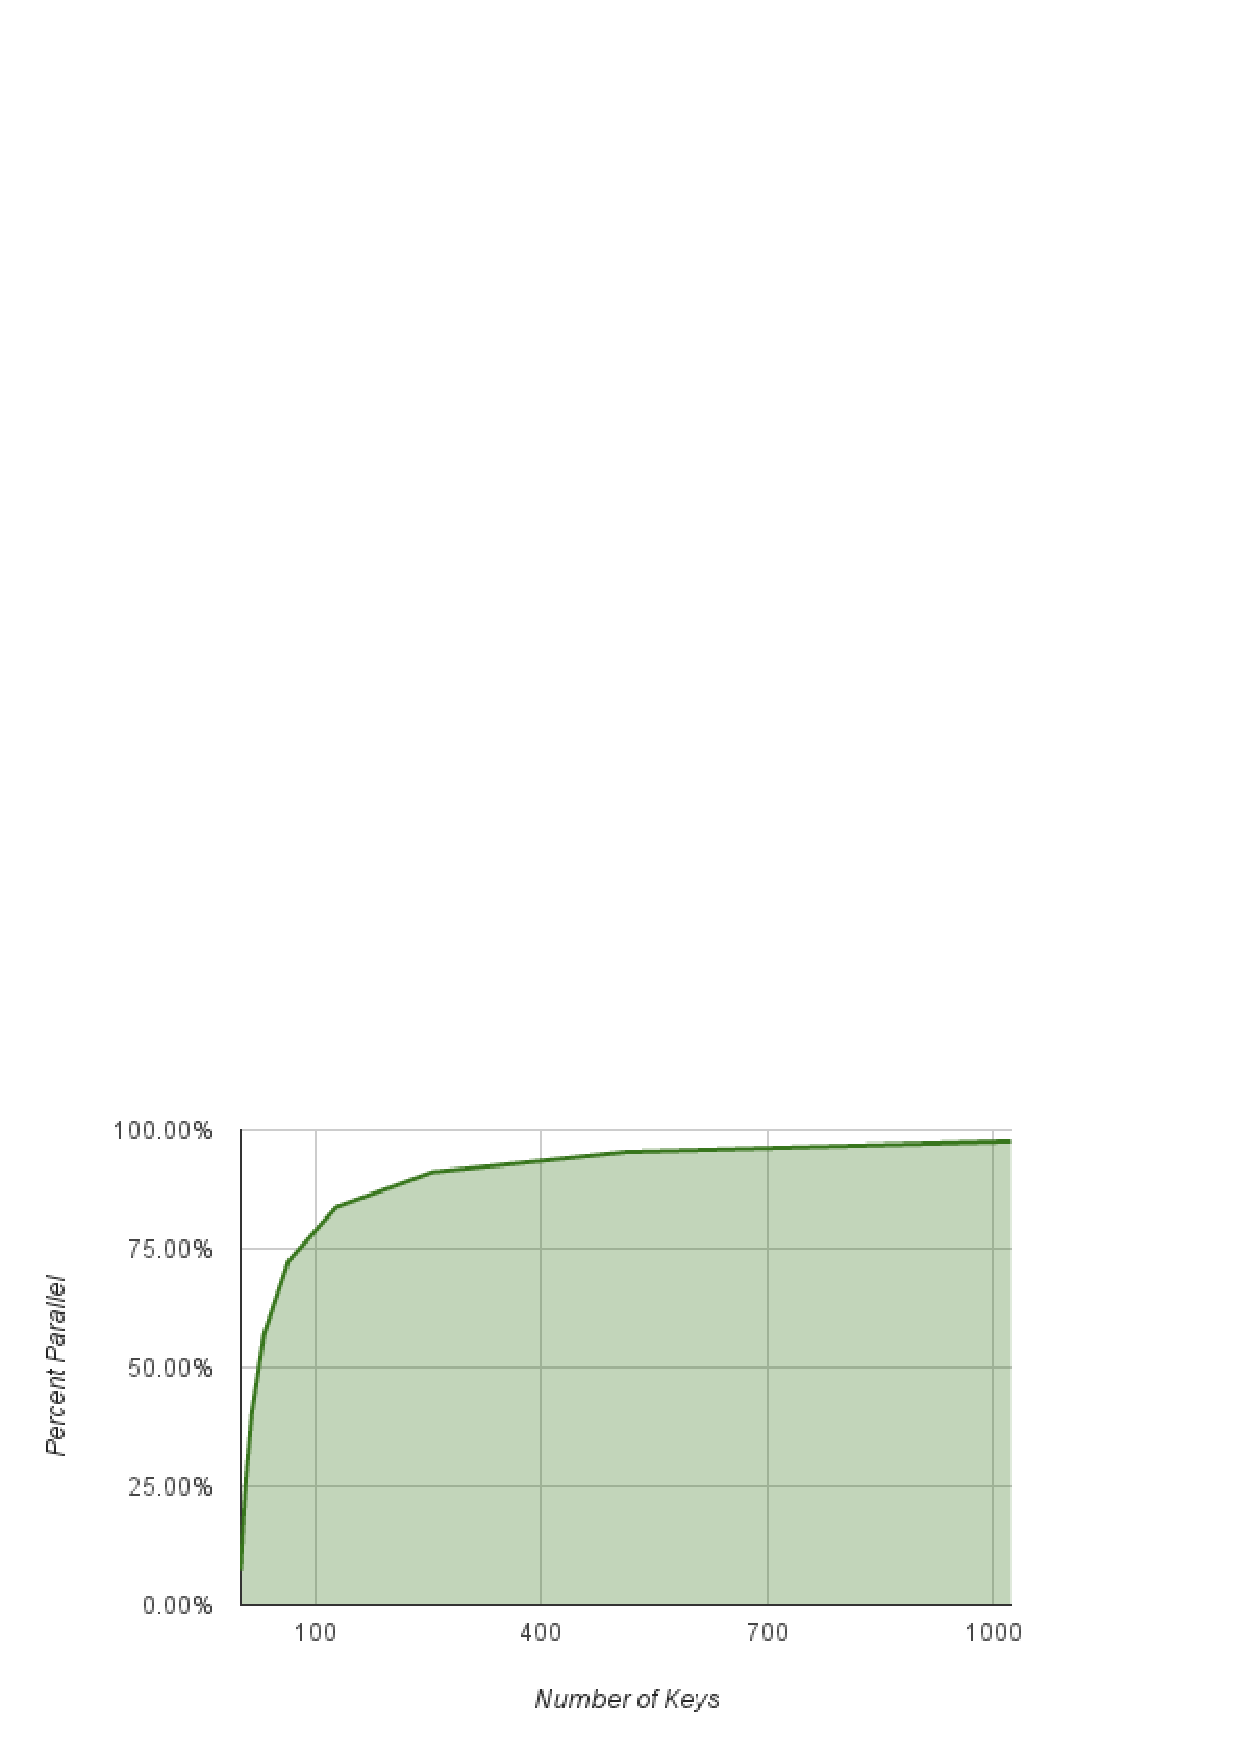
\includegraphics[width=3.5in]{chart_7.png}
   \caption{Total percentage of CUDA implementation that is parallel}
   \label{fig:parPercent}
\end{figure}

\section{Problem Description}
The RSA weakness described above demands that each key in a set be 
compared with each other key to determine if a GCD greater than 1 exists for 
any pair. Given a known set of keys, it is not known before processing 
the keys which will be likely to have a GCD greater than 1; therefore, there 
is no way to eliminate comparisons between specific pairs. The natural 
organization to fulfill this requirement is a comparison matrix of the all 
keys. Each location in the matrix corresponds to a comparison between two 
keys.

\section{Implementation}
\subsection{Problem Decomposition}
Initially, the comparison matrix seems to be an $n^2$ solution. However, the 
diagonal of the matrix created consists of unproductive GCD calculations since 
these entries would compare each key with itself. Furthermore, the matrix is 
symmetrical over the diagonal. Thus, only the comparisons comprising one of 
the triangles needs to be performed. Specifically, 
\begin{equation}
   \label{eq:gcd}
   \mbox{Total number of GCD compares} = \sum_{i=1}^k i
\end{equation}
This reduction in number of overall compares decreases the work 
performed significantly, shown in Figure \ref{fig:compvkeys}. 

\begin{figure}
   \centering
   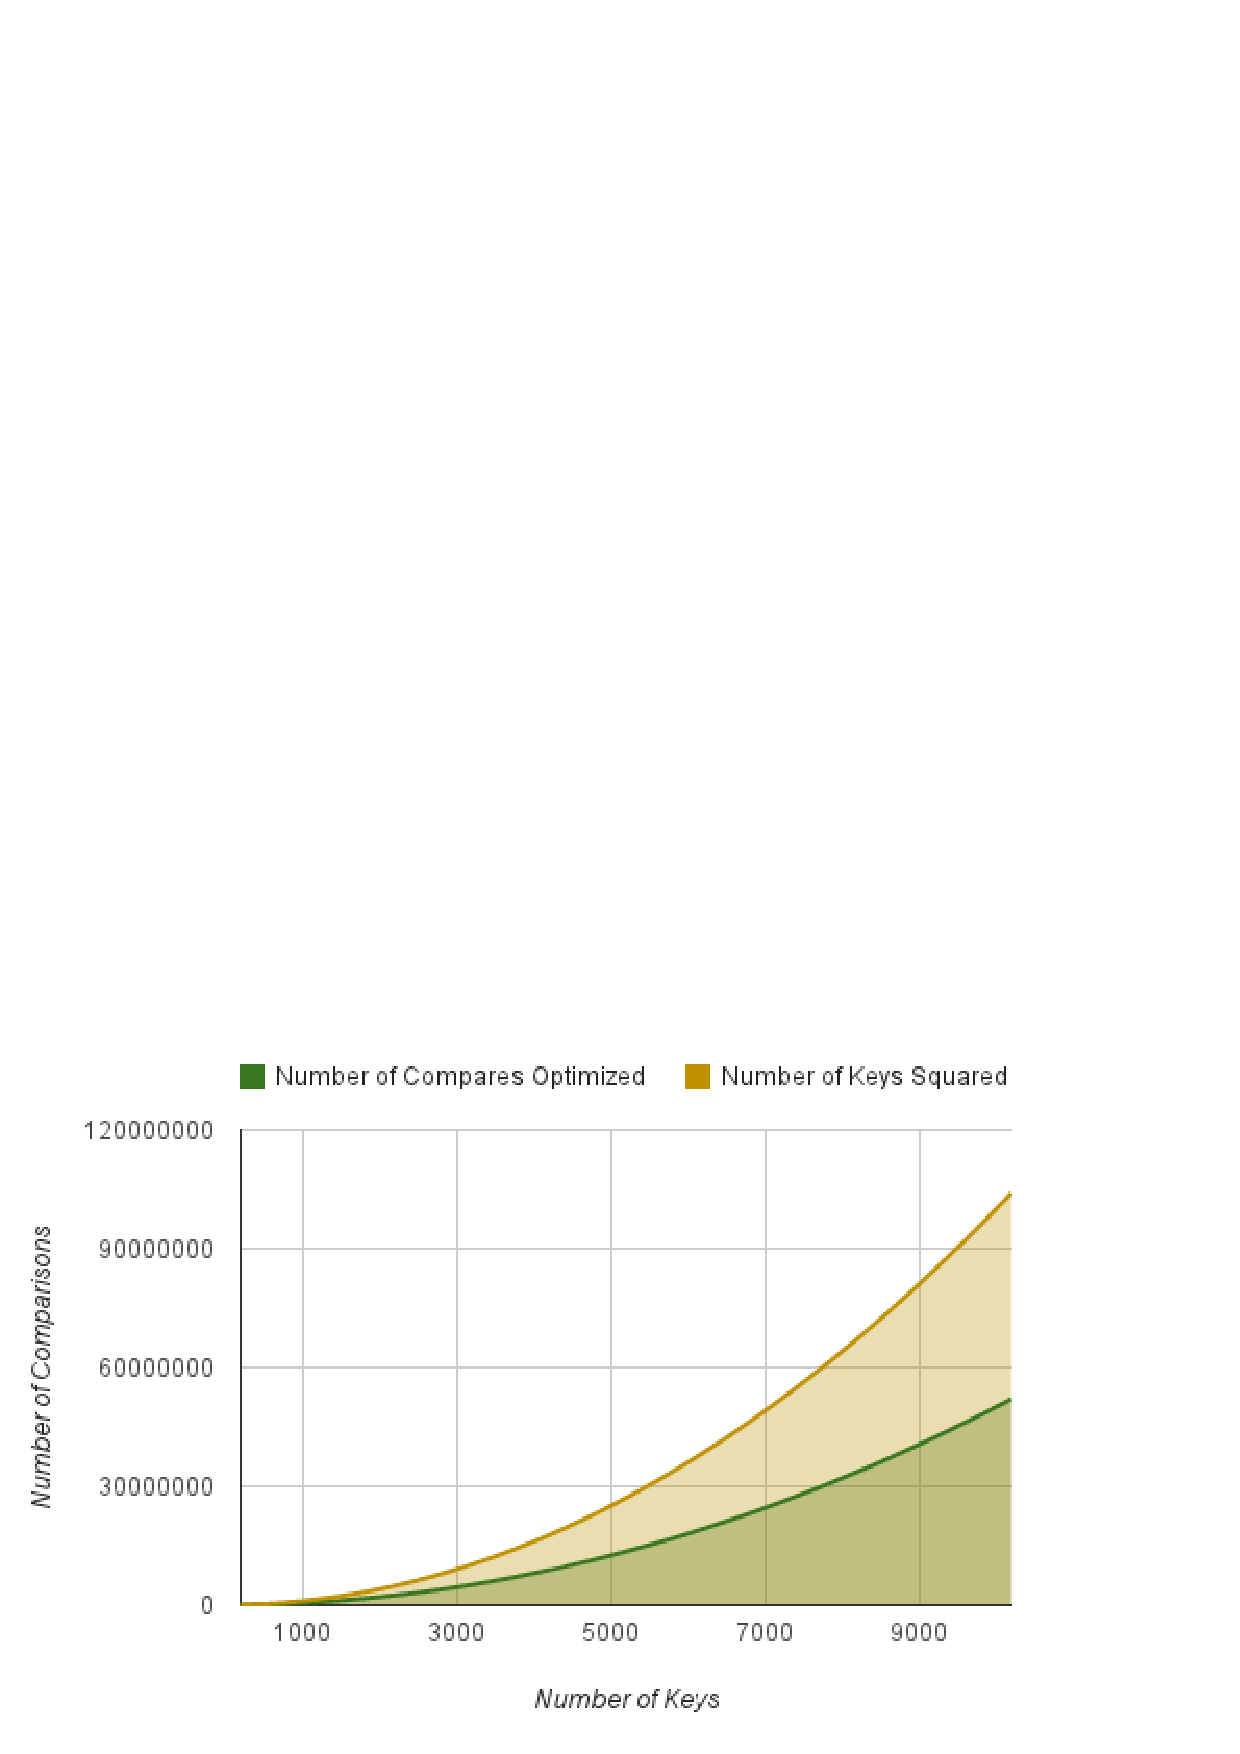
\includegraphics[width=3.5in]{chart_6.png}
   \caption{Number of comparisons needed vs. total number of keys in set}
   \label{fig:compvkeys}
\end{figure}

\subsection{Grid Organization}
\label{sec:GridOrg}
One of the most important aspects of any CUDA implementation is the 
organization of the thread and block array to ensure that the architecture is 
appropriately used to its full potential. The thread array in this 
%JW%
implementation was organized using 3 dimensions. The $x$ dimension represented 
the sectioning of a 1024-bit value into individual 32-bit integers, of which 
there are 32. 
\begin{displaymath}
   \frac{1024 \:\mbox{bits per key}}{32 \:\mbox{bits per integer}} = 
   32 \;\mbox{integers per key}
\end{displaymath}
The remaining dimensions, $y$ and $z$, were set to 4, resulting in a block of 
512 threads. This design decision was experimentally determined. See 
$\S$\ref{sec:Occupancy} for details about Occupancy optimizations.
\begin{displaymath}
   32 \cdot 4 \times 4 = 512
\end{displaymath}
This ensured that each block remained square for algorithmic 
symmetry and simplicity. The $y$ and $z$ dimensions corresponded to how many 
specific keys within the list of all keys were being compared per block. 
Thus, two 1024-bit keys were loaded into each 32-thread warp, which was 
then processed simultaneously as a single comparison. The $x$ dimension was 
chosen for two reasons: 1) so one thread in this dimension would represent 
each of the 32-bit integers inside the key and 2) because there are 32 threads 
in a single warp. Therefore, this thread-array organization ensured that 
compares were done using two entire keys (separated into 32 pieces) that were 
scheduled to the same warp. This eliminated warp divergence since every warp 
was filled and executed with non-overlapping data.

Blocks were arranged in row-major order based on the key comparisons that they 
held. The formula for the number of blocks, $B$, needed for a vector of keys of 
size $k$ can be seen in Equation \ref{eq:blocks}.
\begin{equation}
   \sum_{i=1}^{\left\lceil \frac{k}{4} \right\rceil}i = B
   \label{eq:blocks}
\end{equation}

The limit for a grid in a single dimension is $2^{16} - 1 = 65535$ 
and limits the amount of keys that can be processed to $1444$. To increase 
the number of blocks available for computation, a second grid dimension was 
added. This increased the theoretical maximum number of keys per kernel 
launch as seen in Equation \ref{eq:maxKeys}.
\begin{equation}
   \begin{split}
   \sum_{i = 1}^{\left\lceil\frac{k}{4}\right\rceil} i & \leq {\left(2^{16} - 
   1\right)}^2\\
   k & \leq 370716\\
   \end{split}
   \label{eq:maxKeys}
\end{equation}

\subsection{Shared Memory}
Shared memory was used to load the necessary keys from global memory. Two 
arrays were created in shared memory, representing the thread-array; both 
3-dimensional, $32\times4\times4$ and had an integer loaded into each 
available space. Each array represented which integers would be compared at 
each location in the matrix. A side effect of this organization was that each key would be 
repeated 4 times within its integer array. However, this greatly simplified 
the GCD algorithm so that only a look-up into each array was needed. Since 
shared memory was not the limiting factor for occupancy, it was not a priority 
to optimize this aspect of the design and implementation. 

Shared memory was also used within the GCD algorithm, specifically in the 
greater-than-or-equal-to function, and the subtract function. In the 
greater-than-or-equal-to function, a single integer was allocated for each 
comparison within a block. Within the subtract function, shared memory was 
utilized to represent the borrow value for each integer. 

\subsection{Occupancy}
\label{sec:Occupancy}
Each SM can be assigned multiple blocks at the same time as long as there are 
enough free registers and shared memory available. The ratio of active warps 
to the maximum number of warps supported by a SM is called \emph{occupancy}. 
On the Fermi architecture, the maximum occupancy is achieved when there are 48 
active warps running on a SM at one time. Greater occupancy gives a SM more
opportunities to schedule warps in a fashion to hide memory accesses, thus,
saturating a SM with many warps decreases performance impact. CUDA Fermi cards
have a total of 32768 registers and 49152 bytes of shared memory per SM. The
implementation here uses 17 registers and 4762 bytes of shared memory per
block and therefore results in a maximum occupancy of 100\%.

By using the CUDA occupancy calculator provided by NVIDIA (cf. 
\cite{nvidia2012gpu}), a plot can be formed comparing the threads per block 
with occupancy. To maintain the same block organization outlined above, the 
block dimensions can be $2\times2, 3\times3, 4\times4, 5\times5$ or 128, 228, 
512, 800 threads, respectively. Table \ref{tab:occupancy} shows the calculated 
occupancy for these block sizes. A block size of 512 threads was chosen 
because it results in the greatest occupancy and thus the best performance. 

\begin{table}
%\tbl{Table giving occupancy for various block dimensions\label{tab:occupancy}}{
   \centering
   \begin{tabular}{l|rrrr}
      Threads per block & 128 & 288 & 512 & 800\\
      \hline
              Occupancy & 67\% & 94\% & 100\% & 52\%\\
   \end{tabular}
   \caption{Table giving occupancy for various block 
     dimensions\label{tab:occupancy}}
 
\end{table}

\subsection{Bit-vector}
The initial approach was to allocate a large, multi-dimensional array of 
integers that would hold the results of the CUDA GCD calculations. This was 
allocated to the GPU, so each thread could have access as needed; however, 
since the number of results grew at $n^2$, the lack of scalability in this 
approach was quickly apparent. Additionally, performance decreased due to the 
large array that was being sent over the PCIe bus. Memory transfers to 
the GPU are slow, and must be minimized.

After more careful consideration, a new approach was implemented. There would 
only be a single bit allocated per key-compare to mark whether or not the pair 
had a GCD greater than 1. In this way, only 2 bytes (16 bits = 1 bit per 
compare) were necessary per block ($4\times4 = 16$ compares per block), as 
opposed to the previous $16 \cdot 32 \cdot 4 = 2048$ bytes. Despite not having access 
to the answer immediately after returning from the kernel calculation, this 
approach would be more efficient since there would be a theoretically small 
number of keys that actually returned with GCDs greater than 1 (i.e. the flag 
was set). This small set could then be re-processed (GCDs calculated) using a 
different kernel or using a CPU algorithm. Efficiency would also be increased 
due to the time saved in memory transfers since there was significantly less 
memory to transfer before calling the kernel.

\section{Experimental Setup}
\subsection{Test Machine}
All performance measurements were made on a single machine with an Intel Xeon 
W3503 dual-core CPU and 4 GB of RAM. This machine has one NVIDIA GeForce
GTX 480 GPU with 480 CUDA cores and 1.5 GB of memory. The CUDA driver 
version present on the machine is 4.2.0, release 302.17, the runtime version is
4.2.9. The CUDA compute capability is version 2.0, and the maximum threads per 
block is 1024, with each warp having 32 threads.

\subsection{Reference Implementations}
In order to check the accuracy of the final implementation, as well as to 
provide a point of comparison for benchmarking, two reference implementations 
of this exploit were created. Each was able to use the same format key 
databases (described in $\S$\ref{sec:testSets}). 

The first implementation was written purely in Python using the open source
PyCrypto cryptography library. % 2.7.1. 
%Since Python's 
%\texttt{long} type can contain integers of arbitrary size, and its math library 
%can perform operations on these values, it was most straightforward to 
%implement the entire program using these tools. The open source PyCrypto\footnote{https://www.dlitz.net/software/pycrypto/} 
%library (version 2.5) was used to import and process the RSA key pairs. 
This 
implementation was able to perform the entire exploit, from finding 
weak 1024-bit RSA 
public keys through generating the discovered private keys. 
%It was used 
%primarily as a sanity check for the database generation in order to 
%determine if the keys generated as expected. 
This implementation was not used for performance 
comparison as it was dissimilar to the other two implementations.

A sequential version of the binary GCD algorithm was implemented to serve as a 
second validation tool for the CUDA implementation. This version sequentially 
processed the same input as both other implementations and produced output of the 
same format. Comparison with this implementation ensured that unexpected errors 
did not result merely from processing the data in parallel.

\subsection{Test Sets}
\label{sec:testSets}
In order to conduct meaningful tests, it was necessary to use an identical 
data set in all tests. To facilitate this, a tool was written in Python to 
generate both regular and intentionally weak RSA key pairs using PyCrypto and store them in an SQLite3 database. All keys were generated with a 
constant $e$ of 65537, chosen because this was discovered to be a commonly used 
value (cf. \cite{lenstra:ron}).

The generation process produced a database of RSA key pairs. 
Intentionally weak keys were evenly distributed. 

In order to generate a weak key, this program would generate an initial 
normal RSA key but save the prime used for $p$. For each subsequent bad key, 
$p$ would be replaced with this constant, and $n$ was recalculated. The 
result was that each weak key would have a GCD greater than 1 when 
tested against any other weak key. 

Using this tool, it was possible to build arbitrarily large test sets with a 
known number of keys exhibiting the weakness. When these databases 
were processed using any of the reference implementations, the 
discovered number of weak keys could be directly compared with the 
number of keys expected to be found. This allowed both repeatable testing to 
measure run time, and a method to validate the parallel algorithm was indeed 
finding GCDs as expected. 

\section{Results}
The accuracy of the parallel implementation was verified against the 
sequential implementation by using identical test data sets with known 
weak keys. Since both implementations found the same set of compromised keys,
it was validated that these two implementations 
were internally consistent. Furthermore, both matched the results of the 
separate Python reference implementation: supporting the assertion of accurate 
functionality. The speedup of the CUDA implementation (seen in Figure 
\ref{fig:speedup}) was calculated by comparing its run time with that of the sequential 
implementation. Compare this 
with Figure \ref{fig:parPercent}: this similarity is evidence of the 
implementation presented here matching with theoretical expectations.

\begin{figure}
   \centering
   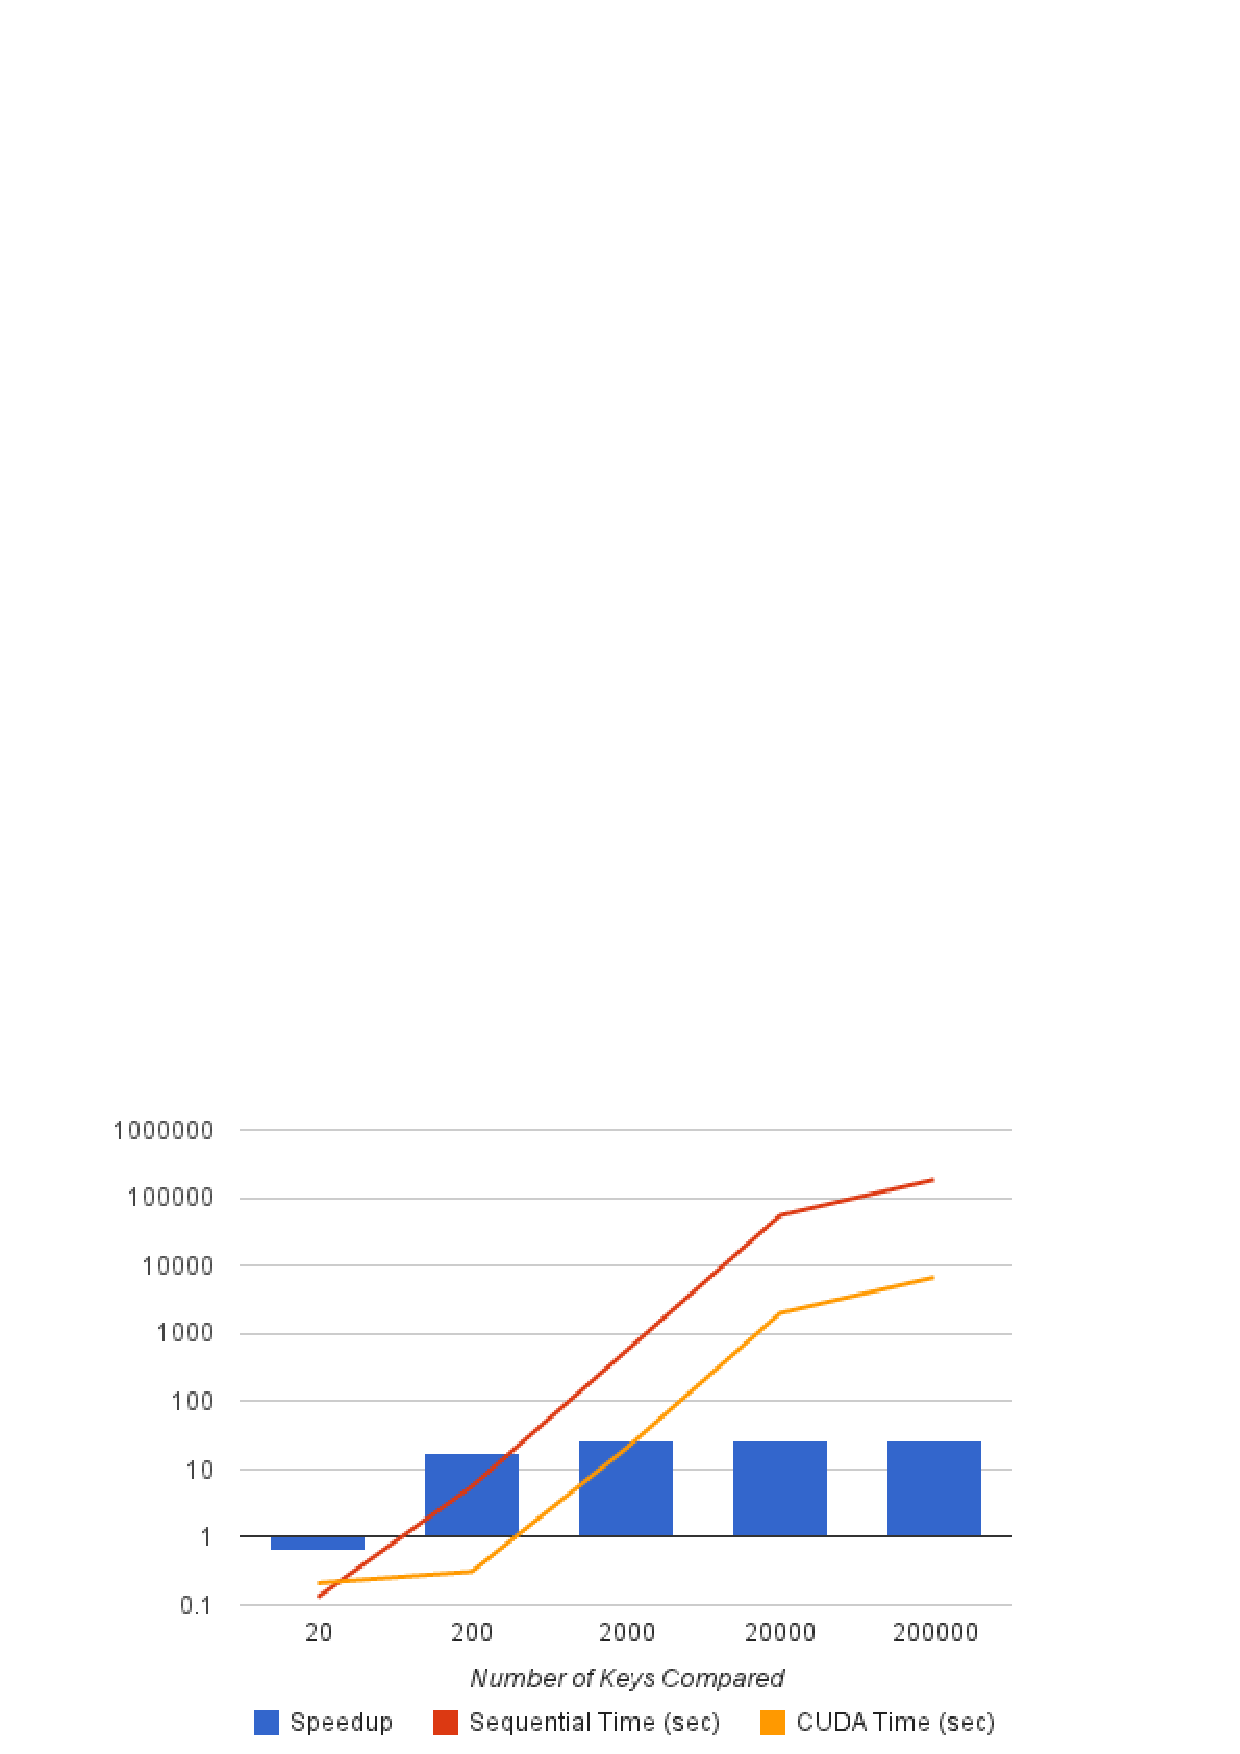
\includegraphics[width=3.5in]{chart_1.png}
   \caption{Speedup of CUDA Implementation to Sequential C++}
   \label{fig:speedup}
\end{figure}

Figure \ref{fig:speedup} shows that speedup increases dramatically with 
the number 
of keys until about 2000 comparisons. At this point, the GPU becomes saturated 
with enough blocks to fully occupy all of the SMs. Speedup remains constant at
27.5 for up to 200000 keys. We have no data beyond this number of keys due to 
the very long run time of the sequential implementation. 

%The increase in the number of 
%comparisons affects the sequential performance significantly more than the CUDA 
%performance, which is particularly apparent in Figure \ref{fig:runtimes}.
%
%\begin{figure}
%   \centering
%   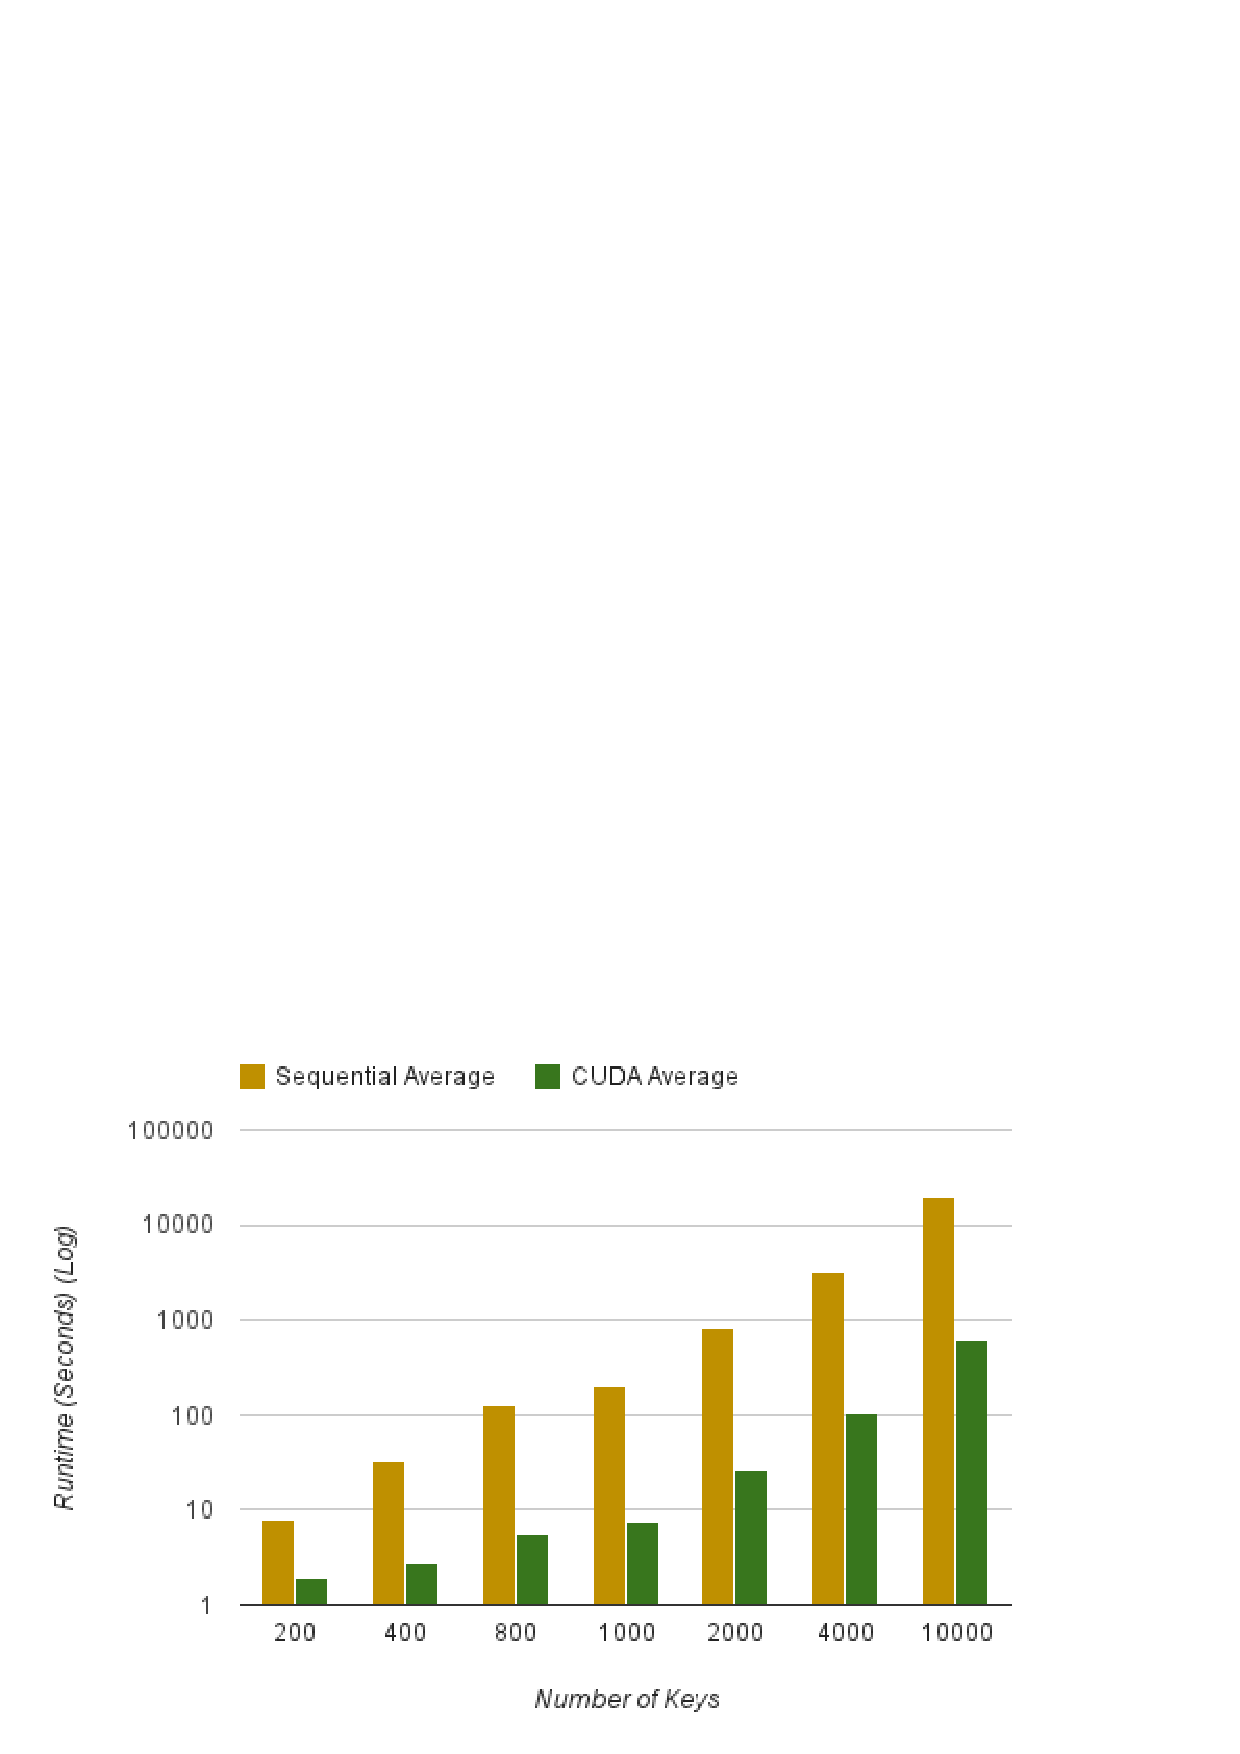
\includegraphics[width=3.5in]{chart_4.png}
%   \caption{Run-time comparison}
%   \label{fig:runtimes}
%\end{figure}

%\begin{table*}
%%\tbl{Average run-times of sequential and CUDA implementations\label{tab:runtimes}}{
%   \centering
%   \begin{tabular}{|l|*{7}{r}|}\hline
%      Number of Keys     & 200 & 400 & 800 & 1000 & 2000 & 4000 & 10000\\
%      \hline
%      Sequential Average (sec) & 8.10 & 32.44 & 129.83 & 202.97 & 810.86 & 8242.75 & 20258.75\\
%      CUDA Average (sec) & 1.97 & 2.71 & 5.47 & 7.64 & 26.31 & 104.15 & 609.11\\\hline
%      \textbf{Speedup} & 4.1 & 11.96 & 23.76 & 26.58 & 30.81 & 31.13 & 33.26\\\hline
%   \end{tabular}
%   \caption{Average run-times of sequential and CUDA 
%     implementations\label{tab:runtimes}}
%\end{table*}

\begin{table*}
%\tbl{Average run-times of sequential and CUDA implementations\label{tab:runtimes}}{
   \centering
   \begin{tabular}{|l|*{5}{r}|}\hline
      Number of Keys        & 20   & 200  & 2000   & 20000    & 200000 \\ \hline
      Sequential Time (sec) & 0.13 & 5.59 & 550.69 & 55121.86 & 185551.91\\
      CUDA Time (sec)       & 0.21 & 0.31 & 20.21  & 2005.09  & 6748.23\\\hline
      \textbf{Speedup}      & 0.6  & 18.0 & 27.2   & 27.5     & 27.5\\\hline
   \end{tabular}
   \caption{Run-times of sequential and CUDA implementations\label{tab:runtimes}}
\end{table*}

%One run of the CUDA implementation was performed using a data set of 200,000 
%keys. Using Equation \ref{eq:gcd}, this many keys required 20,000,100,000 
%comparisons. This run of the program took approximately 114 minutes to 
%complete, which translates to 
%\begin{displaymath}
%   \begin{split}
%      \frac{20,000,100,000 \;\text{comparisons}}
%      {114 \;\text{min}} = 2.923 \times 10^6 \frac{\text{comparisons}}{\text{sec}}
%   \end{split}
%\end{displaymath}
%Each comparison consists of performing the binary GCD calculation between two 
%1024-bit values.

\section{Conclusion}
A large speedup resulted directly from writing a CUDA 
implementation when compared to the sequential implementation. Many 
more keys are able to be compared in a given amount of time using the CUDA
implementation. 

A tool was developed to efficiently and completely compare a list of 1024-bit 
RSA public keys, avoiding repetition and unnecessary work. This 
tools allows an increased number of keys to be compared 
compared to prior work, in turn allowing overall execution time to decrease due 
to the increased parallelism.

The tool described in this paper offers significant advantages over other GCD 
algorithms in CUDA, and practically applies this for comparison of 1024-bit 
RSA keys in order to test for a particular weakness. There also exist 
several areas where the implementation would benefit from further 
investigation and development including application of the GCDs, and 
expansion to iterative kernel calls in order to handle even larger sets of 
keys to compare.

\section{Future Work}
The primary limiting factor of this implementation is the amount of memory 
available on the GPU. Since all key combinations must computed to expose any 
potential weakness, the kernel was structured to take a single vector of 
keys and perform all possible comparisons. In order to process more keys, 
either a GPU with more memory must be used, or the algorithm must be modified 
in order to use multiple, iterative kernel launches. The iterative kernel 
approach would require memory to be separated into two sections that could 
each be filled with subsections of the large, complete array of keys. All 
comparisons would then be performed between the two subsections by calling the 
kernel that is currently implemented. Upon returning from the kernel, the data 
in one subsection would be shifted, and all the compares would then be done 
for those two sets of keys. This process would continue until both vectors 
have iterated over all keys: specifically, the kernel call would reside in a 
pair of nested \texttt{for} loops. This change would allow the implementation 
presented here to process an arbitrary number of keys.

To further enhance the above proposed addition, asynchronous memory 
transfers could also be added to the implementation. When combined with 
multiple kernel launches, a significant portion of the memory I/O (which is one 
of the main limiting factors of performance using the GPU) would be able to be 
masked by simultaneously processing the data currently on the GPU while new 
data is being copied onto it.

An aspect that was originally intended for this project, but was not 
implemented was to have the CUDA kernel return the actual GCD of any keys that 
were found to be ``weak'' in the sense there existed a GCD greater than 1. 
Since a large majority of the GCDs found by our implementation are equal to 
one, memory is wasted if all the results are transferred back to the host. The 
most memory efficient solution would include dynamically allocating memory for 
any significant results on the device. This would remove the recalculation step 
in the current implementation needed to produce private keys.

Recently NVIDIA has released information about a new GPU architecture called 
Kepler\cite{nvidiakepler}.
The Kepler architecture introduces new features that may increase the 
performance of this implementation. \newpage A feature known as Dynamic Parallelism 
allows a CUDA kernel to launch new kernels from the GPU. This would allow 
dynamic allocation of block sizes for different areas of the comparison matrix 
and remove idle threads from the kernel. Hyper-Q is a new technology that 
manages multiple CUDA kernels from multiple CPU threads. With the current 
Fermi architecture, only one CUDA kernel may run on the device at one time. 
This can lead to under utilization of the GPU hardware. An approach using 
multiple CPU threads, each running their own CUDA kernel, could greatly 
increase throughput.

The final missing component of this implementation would be to complete the 
algorithm and use the GCDs which are being calculated to generate RSA private 
key pairs. In order to do this, a heterogeneous multi-process approach may be 
most straightforward. After the parallel run completes, the bit-vector of 
results would be examined to find the key pairs which produced GCDs greater 
than one. In these cases, the GCD would be recomputed, and used as either $p$ 
or $q$. Once this was done, the missing prime would be computed, then based on 
this, $d$ would be found. The resulting RSA public/private key pair could be 
exported or stored for later verification.

%\bibliographystyle{acmsmall}
\bibliographystyle{IEEEtran}
\bibliography{references}

\end{document}
